\section{Introduction}
\label{sec:introduction}

\subsection{Context}
Trident is a small differential-drive robot that I designed and built for a robotics task of
the WorldSkills competition. The task has two parts. The robot first follows a black line on
the floor. It then enters an area in which plastic coins, cylinders about 40\unit{mm} across
and 15\unit{mm} high, each of one colour, have to be carried to the bin of the same colour.
The first part is solved with an infrared reflectance array, the second with a camera, so the
task combines line following with vision-based navigation and a simple manipulation.

The project has passed through two versions.
\begin{enumerate}
  \item \textbf{Version 1} was a test rig: a laser-cut acrylic base with a lidar and a depth
        camera, built to learn ROS~2 and Gazebo and to see the same software run on real
        sensors (\cref{sec:evolution}).
  \item \textbf{Version 2} is the competition robot (\cref{fig:v2-intro}). Its chassis and
        gripper were designed in SolidWorks and printed, and the mechanical design and the
        electronics were completed in fifteen days before the state round of the
        competition.
\end{enumerate}
The robot won the district round. In the state round it did not complete the task, because
its infrared array stopped working. This report documents the design of Version 2 and a
simulation of it in which the whole task is carried out autonomously.

\begin{figure}[htbp]
  \centering
  \begin{subfigure}[b]{0.47\linewidth}
    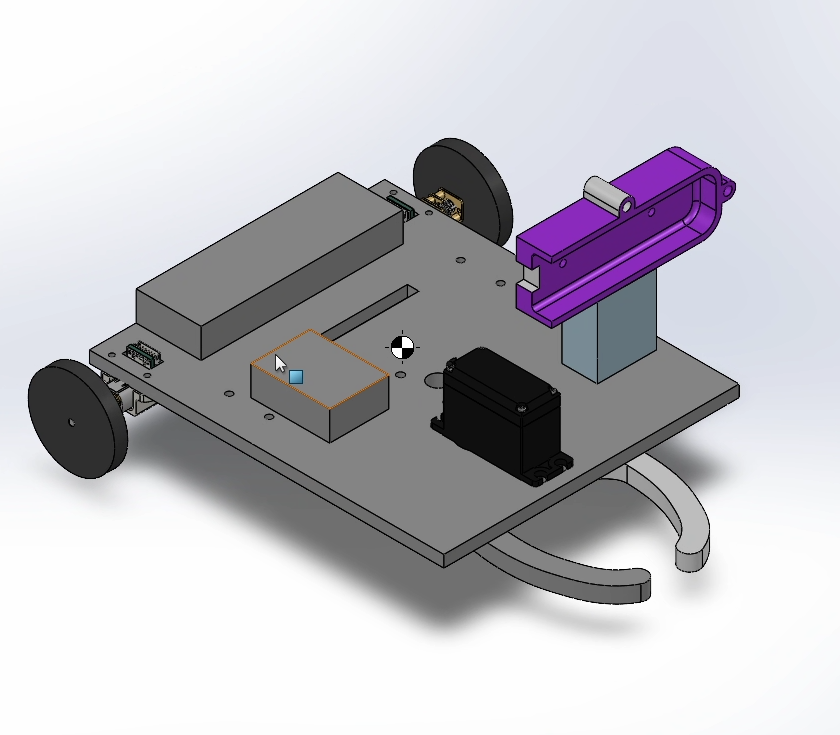
\includegraphics[width=\linewidth]{cad_iso.png}
    \caption{CAD model}
  \end{subfigure}\hfill
  \begin{subfigure}[b]{0.44\linewidth}
    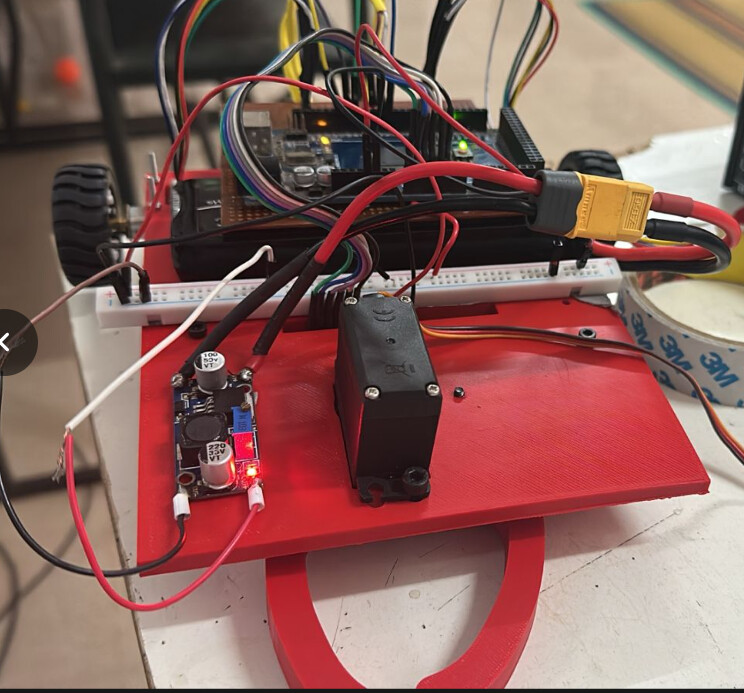
\includegraphics[width=\linewidth]{v2_hardware.jpg}
    \caption{Printed robot during wiring}
  \end{subfigure}
  \caption{Version 2 of Trident: two driven wheels at the rear, a ball caster under the plate
  and a pair of geared jaws at the front. The holder at the side of the plate carries the
  depth camera.}
  \label{fig:v2-intro}
\end{figure}

\subsection{Problem Statement and Objectives}
A robot of this size has little room for mechanism, and a robot built in two weeks has
little time for trial runs. Both facts push decisions into the design: the gripper has to
work without a lift axis and without feedback, and the software has to be tested before the
hardware is free for it. The work reported here therefore has two objectives:
\begin{enumerate}
  \item to design a chassis, a drive and a gripper that move a coin of known size reliably
        with one servo and no sensing in the jaws;
  \item to build a simulation of the robot, from the same CAD model, in which the complete
        mission can be run, scored against ground truth and repeated under varied conditions.
\end{enumerate}

\subsection{Contributions}
The contributions of this report are:
\begin{itemize}
  \item the mechanical design of the robot: its layout, drive, sensor placement and a
        gripper that cages a coin between two curved jaws and slides it along the floor
        (\cref{sec:mechanical});
  \item an analysis of that design from the mass properties of the CAD model, which gives
        the wheel loads, the traction limit and the tipping margin, and which points to
        two improvements of the layout (\cref{sec:mass});
  \item a simulation model of the robot for Gazebo, built on the CAD export, with models of
        the depth camera, the inertial sensor and the infrared array
        (\cref{sec:simulation});
  \item a mission arena whose floor markings are dimensioned from the pitch of the infrared
        array (\cref{sec:arena});
  \item an autonomy stack that combines an existing visual SLAM system and navigation
        framework with a line follower, docking sequences and a mission state machine
        written for this robot (\cref{sec:autonomy});
  \item measurements of the simulated mission over repeated runs with different coin
        orders and obstacle layouts (\cref{sec:results}).
\end{itemize}
I am the sole author of the design, the hardware and the software. Where the software uses
existing open-source packages, \cref{sec:autonomy} states which.

\subsection{Organisation}
\Cref{sec:related} places the work in context. \Cref{sec:evolution} describes the two
versions. \Cref{sec:mechanical,sec:electronics} give the mechanical design and the
electronics. \Cref{sec:simulation,sec:arena} describe the simulation model and the arena,
and \cref{sec:autonomy} the autonomy stack. \Cref{sec:results} reports the measurements,
\cref{sec:verification} the tests, and \cref{sec:discussion} the limitations.
